\documentclass[10pt,twocolumn]{article}

\usepackage[letterpaper,margin=0.70in,columnsep=0.22in]{geometry}
\usepackage{amsmath,amssymb}
\usepackage{graphicx}
\usepackage{booktabs}
\usepackage{array}
\usepackage{url}
\usepackage[colorlinks=true,linkcolor=black,citecolor=black,urlcolor=black]{hyperref}
\usepackage{placeins}

\graphicspath{{../../}{../../results/}{../}{../onboard/figures/}{figures/}}
\setlength{\parindent}{1em}
\setlength{\parskip}{0pt}
\setlength{\textfloatsep}{8pt plus 2pt minus 2pt}
\setlength{\floatsep}{7pt plus 2pt minus 2pt}
\setlength{\intextsep}{7pt plus 2pt minus 2pt}
\renewcommand{\arraystretch}{1.08}
\emergencystretch=2em
\frenchspacing
\raggedbottom

\newcommand{\vect}[1]{\mathbf{#1}}
\newcommand{\mat}[1]{\mathbf{#1}}
\newcommand{\unit}[1]{\hat{\mathbf{#1}}}
\newcommand{\LU}{\mathrm{LU}}
\newcommand{\TU}{\mathrm{TU}}
\newcommand{\ND}{\mathrm{ND}}
\newcommand{\CRTBP}{CR3BP}
\newcommand{\chisq}{\chi^2}

\title{\vspace{-0.35in}Guidance-Coupled Bearing-Only Optical Navigation for Cislunar Transfers}
\author{Varsha Krishnakumar}
\date{May 2026}

\begin{document}

\twocolumn[
\begin{@twocolumnfalse}
\maketitle
\vspace{-0.15in}
\begin{abstract}
Cislunar optical navigation is often validated through estimator-internal statistics, but mission utility depends on the guidance pipeline it feeds.  This paper evaluates the minimum-information case--a single Moon-center bearing stream--through that mission-output lens.  Pixel measurements are converted to tangent-plane line-of-sight residuals, fused with a CR3BP iterated extended Kalman filter (IEKF), and passed to STM-based single-impulse targeting; estimate-driven active pointing closes the measurement-availability loop.  The central claim is that a sparse Moon-center bearing stream is guidance-useful when visibility is actively maintained, but its utility must be judged by terminal miss, NEES, and visibility jointly, and is bounded by explicit dynamical, measurement, and timing assumptions.  In a $1000$-trial CR3BP Monte Carlo the architecture achieves a median terminal miss of $61.6$~km and $99.1\%$ success at the $10^{-3}\,\LU$ screening tolerance; fixed pointing preserves visibility for $24.6\%$ of the tracking arc versus $99.7\%$ under active pointing.  A continuous success-rate-vs-tolerance curve replaces the single-threshold headline.  Six known Robbins-catalog landmarks lift the $39$~km precision-arrival pass rate from $33\%$ to $71\%$; a $3\times 5$ pointing-by-landmark matrix shows landmarks reduce sensitivity to pointing degradation but cannot compensate for visibility loss.  A matched-seed EKF/IEKF/UKF ablation confirms the iteration is not load-bearing at this signal-to-noise.
\end{abstract}
\vspace{0.12in}
\end{@twocolumnfalse}
]

\section*{Nomenclature}
\begin{tabular}{@{}p{0.18\linewidth}p{0.74\linewidth}@{}}
$\vect{x}$ & spacecraft state, $[\vect{r}^T,\vect{v}^T]^T\in\mathbb{R}^6$ \\
$\mu$ & CR3BP mass parameter for the Earth--Moon system \\
$\Phi(t,t_0)$ & state transition matrix (STM) \\
$\vect{P}$ & state-estimation covariance \\
$\vect{Q}_d$ & discrete process-noise covariance \\
$q_a$ & white-acceleration process-noise spectral density \\
$\unit{u}$ & line-of-sight (LOS) unit vector \\
$\vect{E}$ & tangent-plane projection basis for bearing residuals \\
$\vect{H}$ & measurement sensitivity matrix \\
$\vect{R}$ & bearing measurement-noise covariance \\
$\vect{K}$ & Kalman gain \\
$t_c$ & correction-burn time \\
NIS & normalized innovation squared \\
NEES & normalized estimation error squared \\
LU, TU & CR3BP nondimensional length and time units; $1\,\LU=389{,}703.2648$ km \\
\end{tabular}

\section{Introduction}
\label{sec:intro}
Future cislunar missions will operate where ground tracking is valuable but not always sufficient as the only navigation source.  Line-of-sight access is intermittent, antenna resources are shared, and the Earth--Moon geometry leaves updates sparse near mission-design-sensitive phases.  A camera is attractive: passive, lightweight, and already present for inspection, landing, or science.  The limitation is equally important: a single image of a body gives direction, not range.  Bearing-only optical navigation therefore succeeds only if the dynamics and the changing observation geometry supply enough information to recover the missing depth state.

The optical-navigation literature already covers most of the adjacent design space.  Horizon and limb fitting on an extended body provides position, attitude, or both~\cite{christian2021}; surface-feature identification with crater catalogs supports landmark-based fusion~\cite{christianCrater2021,robbins2019}; the JPL deep-space navigation engineering practice is collected in a recent monograph~\cite{owen2024}.  Cislunar-specific studies have evaluated optical observations of natural and artificial targets~\cite{bradley2020}, optical bearings to a single lunar surface landmark in halo orbit~\cite{hinga2023}, optical fusion with radiometric range and Doppler~\cite{ely2021}, and recent flight demonstrations of multi-body optical triangulation~\cite{krause2024}.  Angles-only observability is treated classically by Aidala~\cite{aidala1979} and Nardone and Aidala~\cite{nardone1981}; modern orbital extensions appear in Woffinden and Geller~\cite{woffinden2009} and Geller and Klein~\cite{gellerklein2014}, while Henry and Christian~\cite{henry2023} and Smego and Christian~\cite{smego2025} treat absolute and dynamic triangulation respectively.  Cislunar autonomous-navigation in-flight experience is documented for CAPSTONE~\cite{thompson2022}, and Greaves and Scheeres have studied cislunar maneuver detection and spacecraft-to-spacecraft tracking with optical observables~\cite{greaves2021,greaves2023}.

This paper does not claim a new estimator, measurement model, or flight-readiness result.  The contribution is the guidance-coupled, bounded-realism evaluation of a minimum-information bearing architecture in a cislunar transfer.  The locked thesis is:
\begin{quote}
\emph{A sparse Moon-center bearing stream is guidance-useful when target visibility is actively maintained, but the architecture's utility must be judged by terminal correction performance, NEES, and visibility jointly--not by innovation consistency alone--and is bounded by explicit dynamical, measurement, and timing assumptions.}
\end{quote}
The three guidance-coupled contributions are: (i) a mission-output evaluation framework in which terminal miss, $\Delta V$ inflation, NEES, NIS, and visibility are reported jointly rather than as an estimator-only scorecard; (ii) a quantification of active pointing as part of the navigation architecture, including a $3\times 5$ pointing-degradation by landmark-configuration matrix on matched seeds; and (iii) a bounded-realism characterization through reality checks on terminal tolerance, attitude noise, multi-revolution stability, parallax-vs-range, $\vect{P}_0$ initialization, measurement delay, synthetic and catalog-backed landmarks, and SPICE point-mass truth.  Against the prior literature, the present work is narrow on three axes: the measurement scope is the minimum-information case, the success criterion is mission-output, and the architecture is judged within explicitly bounded assumptions.

The closest published comparison is the Hinga--Williams single-landmark study in a CR3BP-EKF~\cite{hinga2023}, which uses a richer observable than the Moon-center bearing studied here.  Where this work overlaps with Smego and Christian's recent cislunar dynamic-triangulation work~\cite{smego2025}, the difference is in scope: this paper evaluates a guidance-coupled \emph{architecture}, not a state-estimation \emph{algorithm}.  Extended sweeps, detailed sensitivity studies, and the full $q_a$ tuning sweep are reported in the supplemental material; the main paper carries the headline results and the central success-vs-tolerance reframing.

The paper is organized as follows.  Section~\ref{sec:problem} states the problem and the success criteria.  Section~\ref{sec:methods} compresses the dynamics, measurement, IEKF, targeting, active-pointing, and experimental-design building blocks.  Section~\ref{sec:obs} treats bearing-only observability.  Section~\ref{sec:results} presents the baseline Monte Carlo, the active-pointing comparison, the central success-vs-tolerance ECDF, the landmarks-under-pointing-degradation matrix, the estimator ablation, and a bounded-realism summary.  Sections~\ref{sec:discussion} and~\ref{sec:conclusion} discuss limitations and conclude.

\section{Problem Formulation}
\label{sec:problem}

\subsection{Mission Scenario}
The nominal scenario is a southern halo/near-rectilinear halo orbit (NRHO)-class arc near the Earth--Moon $L_2$ region, seeded from the JPL periodic-orbits catalog and visualized with SPICE-backed ephemeris data.  The catalog record sets $\mu=1.215058560962404\times10^{-2}$, $1\,\LU=389{,}703.2648$ km, and $1\,\TU=382{,}981.2891$ s $= 4.43$ days.  The representative tracking arc spans $6.56$ days, approximately one halo period.  All navigation and targeting quantities use nondimensional CR3BP units; the screening tolerance of $10^{-3}\,\LU$ corresponds to approximately $390$ km, and the precision-arrival reality-check threshold of $10^{-4}\,\LU$ corresponds to approximately $39$ km.  Figure~\ref{fig:seed} shows the tracking arc with the Moon and the Earth-relative geometry.

\begin{figure}[t]
\centering
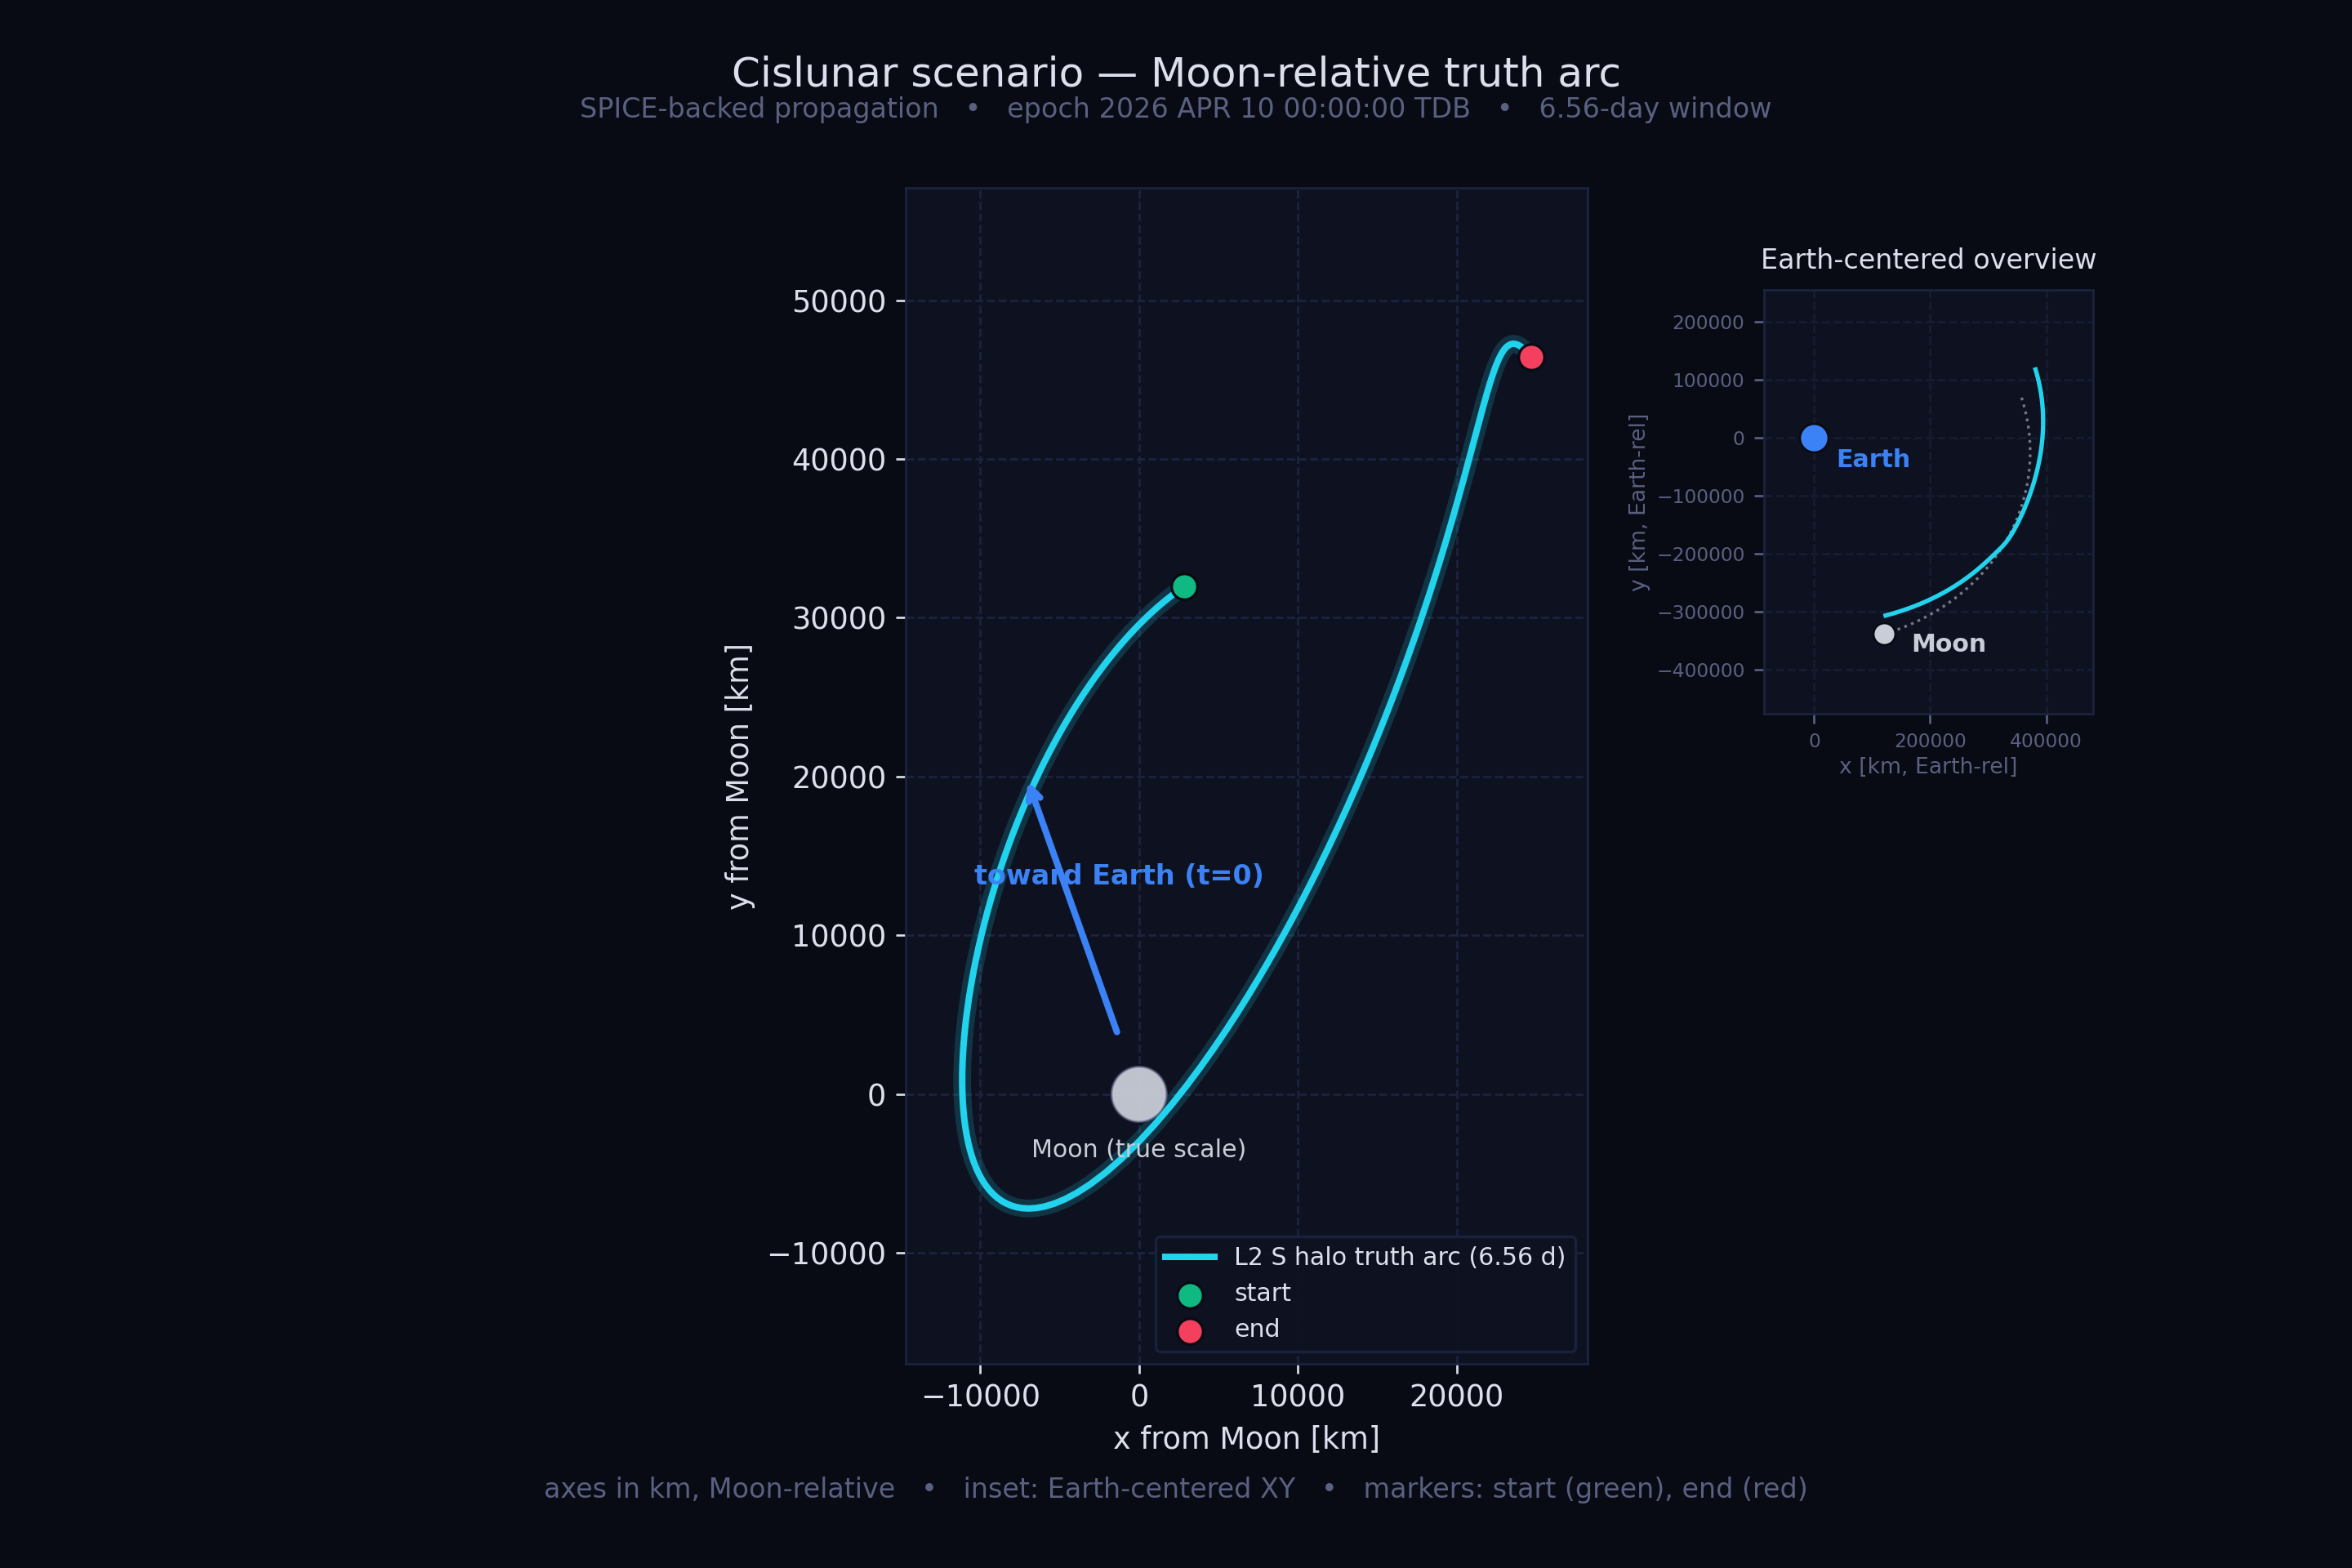
\includegraphics[width=\linewidth]{phase01_slide_visual.png}
\caption{Tracking-arc visualization of the $6.56$-day cislunar window, generated from a SPICE-propagated truth trajectory using DE442s ephemerides in the J2000 inertial frame.  The main panel shows the Moon-relative truth arc with the Moon drawn to scale; the inset shows the Earth-centered geometry.}
\label{fig:seed}
\end{figure}

\subsection{State, Measurement, and Correction Objective}
Given a spacecraft state $\vect{x}=[\vect{r}^T,\vect{v}^T]^T$ evolving under Earth--Moon CR3BP dynamics and a sequence of noisy Moon-center bearing measurements, the estimator produces $\hat{\vect{x}}(t_c)$ and covariance $\vect{P}(t_c)$ at correction time $t_c$.  The guidance objective is to compute a single-impulse estimated-state burn $\Delta\vect{v}_E$ whose terminal miss at $t_f$ is close to the perfect-information burn $\Delta\vect{v}_P$ computed from the true state.  Each accepted image contributes only two angular constraints; range to the Moon and all three velocity components must be inferred through the measurement history and the dynamics rather than measured directly.

\subsection{Success Criteria}
Performance is reported jointly: terminal miss after applying $\Delta\vect{v}_E$ and propagating to $t_f$; the magnitude difference $\|\Delta\vect{v}_E-\Delta\vect{v}_P\|$ and the relative $\Delta V$ inflation; the visibility fraction (the share of scheduled measurement epochs at which a target was inside the field of view and gating allowed an update); the trial-mean NIS and NEES with the diagnostic $\chisq(2)$ and $\chisq(6)$ 95\% bands.  A trial is screened as successful when the post-correction terminal miss is below $10^{-3}\,\LU$; the screening tolerance is intentionally generous and is supplemented by a continuous success-rate-vs-tolerance curve (Figure~\ref{fig:central}) so mission-specific accuracy can be read off directly.

\subsection{SPICE Truth Model}
``SPICE-backed'' refers to truth and visualization products generated with the NASA NAIF SPICE toolkit~\cite{naif} from the DE442s planetary ephemeris and the NAIF leapseconds kernel; inertial states are returned by \texttt{spkezr} in J2000 at TDB epochs anchored to the catalog start time.  The SPICE truth propagator is a Sun--Earth--Moon point-mass three-body integration with $GM_{\rm Sun}=1.32712440018\times 10^{11}$, $GM_{\rm Earth}=3.986004418\times 10^{5}$, and $GM_{\rm Moon}=4902.800066$~$\mathrm{km^3/s^2}$, seeded by converting the dimensionless CR3BP halo state to inertial km/s at the same epoch and integrated with adaptive tolerances.  The estimator dynamics are always CR3BP in the synodic frame; SPICE is used only for truth generation and for scenario visualization.  Lunar non-spherical gravity, solar radiation pressure, propellant-mass changes, attitude actuator dynamics, light-time, and aberration are intentionally not modeled in either arm.

\section{Models and Algorithms}
\label{sec:methods}

\subsection{Dynamics and Process Noise}
The primary filter and targeting experiments use the Earth--Moon CR3BP in the synodic frame.  The primaries are fixed at $\vect{r}_E=(-\mu,0,0)^T$ and $\vect{r}_M=(1-\mu,0,0)^T$; the implemented equations of motion derive from the standard pseudo-potential $\Omega(x,y,z)=\tfrac{1}{2}(x^2+y^2)+(1-\mu)/r_1+\mu/r_2$.  The same CR3BP class computes the Jacobi constant, the variational dynamics matrix $\mat{A}(t)$, and the Lagrange points, giving the estimator a nonlinear propagator and the linearized dynamics needed for covariance transport.

Covariance propagation uses the STM, $\Phi(t,t_0)=\partial\vect{x}(t)/\partial\vect{x}(t_0)$, integrated alongside the state through $\dot{\Phi}=\mat{A}(t)\Phi$, $\Phi(t_0,t_0)=\mat{I}_6$.  A filter step integrates the combined system, unpacks the terminal state and STM, and updates covariance as $\bar{\vect{P}}_{k+1}=\Phi_k\vect{P}_k^+\Phi_k^T+\vect{Q}_{d,k}$ with the Joseph form (Section~\ref{sec:iekf}) for numerical stability.  The discrete process-noise model is white acceleration:
\begin{equation}
\vect{Q}_d(\Delta t)=q_a
\begin{bmatrix}
\frac{\Delta t^3}{3}\mat{I}_3 & \frac{\Delta t^2}{2}\mat{I}_3\\
\frac{\Delta t^2}{2}\mat{I}_3 & \Delta t\mat{I}_3
\end{bmatrix}.
\label{eq:q}
\end{equation}
The canonical operating point adopted for the n=1000 production runs reported here is $q_a=10^{-14}$.  A fine $q_a$ sweep (supplemental material) shows that $q_a=10^{-9}$ would put the trial-mean NEES inside the $\chisq(6)$ 95\% band on $99.4\%$ of trials but slightly inflate the median terminal miss; $q_a=10^{-14}$ trades that NEES band fraction for a tighter linearization regime that exposes more covariance dynamics in the realism sweeps.  The $99.1\%$ screening pass rate is unchanged either way.

\subsection{Optical Measurement and Tangent-Plane Residual}
The camera is modeled as an ideal pinhole with intrinsics $\mat{K}$ (image $640\times 480$ px, $f_x=f_y=400$ px, principal point at the image center, full FOV $77.3^{\circ}\times 61.9^{\circ}$, measurement cadence $0.02\,\TU\approx 2.13$ h).  A pixel detection $(u_{\rm px},v_{\rm px})$ is converted to a normalized camera-frame ray $\unit{u}_C=[(u_{\rm px}-c_x)/f_x,\ (v_{\rm px}-c_y)/f_y,\ 1]^T/\lVert\cdot\rVert$ and rotated into the navigation frame.  The angular noise floor is $\sigma_\theta\approx\sigma_{\rm px}/f_x$, giving a noisy unit LOS vector and a two-dimensional angular covariance.

For a body position $\vect{r}_b$ and spacecraft position $\vect{r}_{sc}$, the predicted LOS is $\unit{u}(\vect{x})=(\vect{r}_b-\vect{r}_{sc})/\lVert\vect{r}_b-\vect{r}_{sc}\rVert$.  An orthonormal tangent basis $\vect{e}_1,\vect{e}_2$ perpendicular to the predicted LOS is stacked as $\mat{E}=[\vect{e}_1\ \vect{e}_2]^T$, and the two-dimensional innovation is
\begin{equation}
\vect{y}_k = \mat{E}\bigl(\unit{u}_{\rm meas}-\unit{u}(\bar{\vect{x}}_k)\bigr).
\label{eq:resid}
\end{equation}
For range $\rho=\lVert\vect{r}_b-\vect{r}_{sc}\rVert$, the LOS sensitivity is $\partial\unit{u}/\partial\vect{r}_{sc}=-(1/\rho)(\mat{I}_3-\unit{u}\unit{u}^T)$, giving the measurement matrix
\begin{equation}
\mat{H}=
\begin{bmatrix}
\mat{E}\,\partial\unit{u}/\partial\vect{r}_{sc} & \mat{0}_{2\times3}
\end{bmatrix},
\qquad
\mat{R}=\sigma_\theta^2\mat{I}_2.
\label{eq:h-bearing}
\end{equation}
The bearing measurement contributes at most two angular constraints per frame; range and velocity must be recovered over time through motion and dynamics.

The baseline measurement model is an idealized body-center bearing.  Illumination-dependent center-of-brightness bias, limb-fitting errors, exposure-and-thresholding effects, and star-field false detections are intentionally excluded so the guidance consequences of a minimal bearing stream can be isolated; the L1/L2 landmark variants (Section~\ref{sec:landmarks-pointing}) extend this to known-identity surface features.

\subsection{Iterated EKF}
\label{sec:iekf}
The estimator is an iterated extended Kalman filter, run from the first measurement epoch onward; no Consider Filter or batch pre-filter is used at startup.  The decision is deliberate: the bearing measurement in Eq.~\eqref{eq:h-bearing} is nonlinear in position even at small initialization errors, the iterated update absorbs this within a single epoch, and the $\vect{P}_0$ scaling sweep (supplemental material) confirms robust convergence up to $100\times$ wider initial covariance.

The IEKF prediction is the STM propagation above.  The measurement update uses the standard innovation covariance $\mat{S}_k=\mat{H}_k\bar{\vect{P}}_k\mat{H}_k^T+\mat{R}_k$ and Kalman gain $\mat{K}_k=\bar{\vect{P}}_k\mat{H}_k^T\mat{S}_k^{-1}$; because the bearing measurement is nonlinear in position, the correction is iterated with re-linearization at each step:
\begin{equation}
\vect{x}^{(i+1)}=\bar{\vect{x}}+\mat{K}^{(i)}\bigl[\vect{y}^{(i)}+\mat{H}^{(i)}(\vect{x}^{(i)}-\bar{\vect{x}})\bigr].
\end{equation}
The covariance is updated with the Joseph form
\begin{equation}
\vect{P}^{+}=(\mat{I}-\mat{K}\mat{H})\bar{\vect{P}}(\mat{I}-\mat{K}\mat{H})^T+\mat{K}\mat{R}\mat{K}^T,
\end{equation}
which is more robust to numerical loss of symmetry and positive definiteness than the simplified update.  The maximum-iteration count is 3 in the IEKF baseline; the EKF/IEKF/UKF ablation (Section~\ref{sec:results-ablation}) sets it to 1 for the EKF cell and shows that the iteration is not load-bearing at the headline operating point.

The estimator is evaluated with both measurement-space and state-space consistency tests:
\begin{equation}
\mathrm{NIS}_k = \vect{y}_k^T\mat{S}_k^{-1}\vect{y}_k,\qquad
\mathrm{NEES}_k=(\hat{\vect{x}}_k-\vect{x}_k)^T\vect{P}_k^{-1}(\hat{\vect{x}}_k-\vect{x}_k).
\end{equation}
NIS should follow $\chisq(2)$ and NEES should follow $\chisq(6)$ under correct modeling; the $\chisq$ bands are used as diagnostic reference levels rather than exact hypothesis tests because measurements along a trajectory are temporally correlated.

\subsection{STM-Based Single-Impulse Targeting}
The guidance pipeline computes a single impulsive correction at $t_c$ that minimizes the terminal position error at $t_f$.  Given the state estimate $\hat{\vect{x}}(t_c)$ propagated forward to a terminal position $\vect{r}(t_f)$, the position-to-velocity STM block $\Phi_{rv}(t_f,t_c)$ maps a velocity impulse $\Delta\vect{v}$ at $t_c$ to a terminal position change $\Phi_{rv}\Delta\vect{v}$.  The correction is the linear-least-squares solution $\Delta\vect{v}_E=-\Phi_{rv}^{-1}(\vect{r}(t_f)-\vect{r}_{\rm target})$; the perfect-information benchmark $\Delta\vect{v}_P$ uses the same STM with the true state at $t_c$.  Performance is measured by terminal miss after applying $\Delta\vect{v}_E$ and the magnitude/direction differences between $\Delta\vect{v}_E$ and $\Delta\vect{v}_P$.

\subsection{Active Pointing as Observability Strategy}
Fixed body pointing is a fragile assumption: if the Moon drifts out of frame, measurements disappear and the filter reverts to open-loop propagation in a strongly nonlinear environment.  The active-pointing policy treats camera orientation as part of the navigation architecture.  At each measurement epoch the current state estimate and the target position define a desired LOS; the camera DCM is commanded along that LOS; truth-side attitude noise (when applied) is composed multiplicatively with the commanded DCM, while the filter back-projects through the unperturbed commanded DCM so that bias, lag, and noise show up as un-modeled measurement-side error rather than as known noise the filter could absorb.  Fixed pointing, ideal estimate-driven active pointing, biased active pointing, lagged active pointing, and attitude-noisy active pointing are all instantiations of this scaffolding; only the commanded DCM and the post-command perturbation differ.

\subsection{Experimental Design}
The headline Monte Carlo uses $n=1000$ deterministic-seed trials per cell with $\sigma_{\rm px}=1$ pixel, no random dropout, estimate-driven active pointing, $q_a=10^{-14}$, and $t_c=2.0\,\TU$.  Initial truth-injection and estimate perturbations are sampled per component from zero-mean Gaussians with $\sigma_r=10^{-4}\,\LU$ and $\sigma_v=10^{-4}\,\LU/\TU$.  The IEKF is initialized with $\vect{P}_0=\mathrm{diag}(10^{-6}\mat{I}_3,10^{-7}\mat{I}_3)$ in $\LU^2$ and $(\LU/\TU)^2$; converted to physical units the per-axis $1\sigma$ initial knowledge is $\sigma_r\approx 390$ m and $\sigma_v\approx 0.32$ m/s, intended as a representative end-of-orbit-determination handoff from a ground-tracking pass into the on-board optical phase.  The $\vect{P}_0$-scale sweep in the supplemental material extends this up to a $100\times$ wider initial covariance and shows the headline result is not a tightness artifact.  All bearing updates use the same gating policy ($\texttt{gating\_enabled}=\texttt{False}$) so accept/reject behavior is comparable across filter and landmark variants.  Reproducibility constants (canonical $1\,\LU$, canonical $q_a$, mission-tolerance thresholds, and the full figure-to-script manifest) live in \texttt{scripts/\_paper\_constants.py} and \texttt{docs/experiment\_manifest.md} in the project repository.

\section{Bearing-Only Observability}
\label{sec:obs}
At a single image time, the tangent-plane bearing measurement is rank-deficient by construction: $\mathrm{rank}(\mat{H}_k)\le 2$.  For position alone, this is the familiar ``missing range'' intuition; for the full six-state problem the instantaneous nullspace is larger because the measurement has no direct velocity sensitivity.  Velocity and range become observable through the time history of CR3BP motion and the way later LOS measurements depend on earlier position and velocity through the STM.

Over an observation arc, the relevant local observability object is the accumulated unweighted Gramian
\begin{equation}
\mat{W}_N=\sum_{k=1}^{N}\Phi(t_k,t_0)^T\mat{H}_k^T\mat{H}_k\Phi(t_k,t_0).
\label{eq:gramian}
\end{equation}
Full rank of $\mat{W}_N$ is a necessary local test, but its conditioning is the more practical metric: a full-rank Gramian can still contain a very weak direction that makes range or velocity slow to recover.  In practice these weak directions correspond primarily to range and to certain velocity components aligned with the line of sight.  The accumulated Gramian for the representative trajectory is locally full rank, but its eigenvalues span roughly seven orders of magnitude, and the weakest mode is concentrated in the in-plane $\{x,y,v_x,v_y\}$ subspace.  The measurement history loses practical observability when LOS direction changes too little, when the relative motion is nearly straight-line over the tracking window, or when pointing or field-of-view limits remove measurements; this is the analytical version of the qualitative statement that early correction times and fixed pointing are fragile.

\section{Results}
\label{sec:results}

\subsection{Baseline Monte Carlo}
\label{sec:results-baseline}
Table~\ref{tab:baseline} summarizes the $n=1000$ baseline at the canonical operating point.  The IEKF correction is not identical to the perfect-information burn, but the navigation error is small enough that the closed-loop correction usually meets tolerance.  The median terminal miss is $1.58\times10^{-4}\,\LU\approx 61.6$~km; the 95th percentile is $5.86\times10^{-4}\,\LU\approx 228$~km, still below the screening tolerance.  The uncorrected median miss is $1.19\times10^{-3}\,\LU\approx 465$~km, so the estimated-state correction improves typical terminal error by a factor of roughly $7.5$.  The trial-mean NIS is $1.94$, close to the $\chisq(2)$ expectation of $2.0$; the trial-mean NEES is $5.78$, with the band-fraction nuance discussed in Section~\ref{sec:discussion}.

\begin{table}[t]
\centering
\caption{Baseline Monte Carlo, $n=1000$, $\sigma_{\rm px}=1$ pixel, estimate-tracking, $t_c=2.0$, $q_a=10^{-14}$.}
\label{tab:baseline}
\scriptsize
\resizebox{\linewidth}{!}{%
\begin{tabular}{@{}p{0.39\linewidth}ccc@{}}
\toprule
Metric & Median & 5th pct. & 95th pct. \\
\midrule
Terminal miss [LU] & $1.58\times10^{-4}$ & $3.22\times10^{-5}$ & $5.86\times10^{-4}$ \\
Terminal miss [km] & 61.64 & 12.56 & 228.27 \\
$\|\Delta\vect{v}_{E}-\Delta\vect{v}_{P}\|$ & $2.91\times10^{-4}$ & $6.47\times10^{-5}$ & $8.15\times10^{-4}$ \\
Relative $\Delta V$ inflation & $+1.15\%$ & $-31.7\%$ & $+51.8\%$ \\
Pos.\ err.\ at $t_c$ [LU] & $4.96\times10^{-5}$ & $1.93\times10^{-5}$ & $1.16\times10^{-4}$ \\
Trial-mean NIS & 1.94 & 1.63 & 2.28 \\
Trial-mean NEES & 5.78 & 2.58 & 24.64 \\
\bottomrule
\end{tabular}}
\end{table}

\subsection{Active Pointing as Architecture}
\label{sec:results-active}
Table~\ref{tab:active} contrasts fixed and estimate-driven pointing on the same $301$-step active-tracking experiment.  The fixed camera preserves visibility for $24.6\%$ of candidate measurement epochs; estimate-driven pointing preserves $99.7\%$.  The fixed case eventually diverges because the filter stops receiving useful measurements; active pointing holds the target near the principal point and keeps the estimator stable.  Active pointing is therefore not an attitude-control detail; it is part of the observability strategy.

\begin{table}[t]
\centering
\caption{Fixed versus estimate-driven active pointing on the $301$-step active-tracking experiment.  Errors are in nondimensional CR3BP units.}
\label{tab:active}
\scriptsize
\begin{tabular}{@{}lccc@{}}
\toprule
Mode & vis.\ fraction & final $|\vect{r}|$ err. & terminal miss \\
\midrule
Fixed & 0.257 & 440.6 & $4.86\times10^{-1}$ \\
Active (estimate-tracking) & 0.997 & $\sim 10^{-4}$ & $\sim 10^{-4}$ \\
\bottomrule
\end{tabular}
\end{table}

\subsection{Central Success-vs-Tolerance Result}
\label{sec:results-central}
The screening tolerance of $10^{-3}\,\LU$ is too coarse for any precision-arrival claim; Figure~\ref{fig:central} reframes the headline as the empirical terminal-miss distribution and a continuous success-rate-vs-tolerance curve over $[1,1000]$~km on the same $n=1000$ matched-seed populations.  Four curves are shown jointly: the CR3BP baseline (Moon-only, active pointing), the SPICE point-mass truth comparison, the CR3BP run with Moon plus six Robbins-catalog landmarks (Tycho, Copernicus, Aristarchus, Plato, Kepler, Grimaldi)~\cite{robbins2019}, and the uncorrected baseline (the same CR3BP trials with no midcourse burn) in grey as a reference for what the guidance pipeline is doing.

\begin{figure*}[t]
\centering

\includegraphics[width=0.95\textwidth]{../../results/mc/phase_h_central_ecdf/06t_success_ecdf_central.png}
\caption{Terminal-miss empirical CDF (top) and success rate as a function of mission-tolerance threshold (bottom) for four $n=1000$ matched-seed populations: CR3BP-truth Moon-only with active pointing (cyan), SPICE point-mass truth Moon-only with active pointing (amber), CR3BP-truth Moon plus L2 Robbins-catalog landmarks (green), and the uncorrected reference (grey, dashed).  Vertical guides mark the screening tolerance ($390$~km) and two precision-arrival reality-check points ($39$~km and $25$~km).  The 390~km threshold is useful as a screening tolerance, but mission-specific accuracy must be read directly from the curve.}
\label{fig:central}
\end{figure*}

\begin{table}[t]
\centering
\caption{Pass rates and distribution summaries for the four central-figure populations, $n=1000$ matched-seed trials each.}
\label{tab:central-pass}
\scriptsize
\resizebox{\linewidth}{!}{%
\begin{tabular}{@{}lccccc@{}}
\toprule
population & $n$ & $<\!25$~km & $<\!39$~km & $<\!390$~km & med / p95 [km] \\
\midrule
CR3BP baseline                   & 1000 & 18.10\% & 32.80\% &  99.10\% &  61.64 / 228.27 \\
SPICE point-mass truth           & 1000 &  6.80\% & 11.20\% &  85.30\% & 182.88 / 539.02 \\
Moon $+$ L2 landmarks            & 1000 & 49.80\% & 71.30\% & 100.00\% &  25.07 /  72.51 \\
Uncorrected (no burn)            & 1000 &  1.60\% &  3.80\% &  41.80\% & 464.67 / 1297.40 \\
\bottomrule
\end{tabular}}
\end{table}

The central message of Table~\ref{tab:central-pass} is the per-tolerance reading: at $390$~km the baseline architecture clears comfortably ($99.1\%$); at the $39$~km reality-check the same architecture lands in a regime where mission-design choices begin to matter ($32.8\%$ CR3BP, only $11.2\%$ under SPICE truth, but $71.3\%$ with landmarks); at $25$~km the corresponding numbers are $18.1\%/6.8\%/49.8\%$.  The uncorrected reference confirms the IEKF correction is doing meaningful work even at the screening tolerance ($99.1\%$ versus $41.8\%$ uncorrected), and substantially more at the tighter tolerances ($32.8\%$ versus $3.8\%$ at $39$~km).

\subsection{Landmarks Under Pointing Degradation}
\label{sec:landmarks-pointing}
A natural advisor question is whether known-landmark availability \emph{reduces dependence on aggressive active pointing}.  We probe this with a $3\times 5$ matrix on matched seeds at $n=1000$ per cell, sweeping landmark configuration $\{$Moon-only, $L_2$ landmarks only, Moon $+$ $L_2$ landmarks$\}$ against pointing mode $\{$fixed, ideal estimate-driven, biased estimate-driven, lagged estimate-driven, attitude-noisy estimate-driven$\}$.  The biased mode applies a $0.1^{\circ}$ constant boresight bias about the camera-frame $y$ axis; the lagged mode tracks the estimate from five measurement steps ago ($\approx 0.1\,\TU$); the noisy mode injects $\sigma_{\rm att}=0.05^{\circ}$ per-step zero-mean attitude noise.  The $L_2$ layout is the six Robbins-catalog craters cited above.

To make the mechanism distinction observable, two per-source quantities are logged in addition to the standard metrics: per-source visibility (the existing $\texttt{valid\_rate\_moon}$ and $\texttt{valid\_rate\_landmarks}$ aggregations) and the median angular offset of each source from the commanded camera boresight.  The angular-offset pair separates the visibility-substitution mechanism (a source remains in the FOV when others do not) from the geometry-improvement mechanism (sources stay close to the boresight while bearing diversity grows).

\begin{table}[t]
\centering
\caption{Landmarks under pointing degradation, $n=1000$ per cell, matched seeds across all 15 cells.  Column block is $\{$\textbf{fixed}, \textbf{ideal} active, \textbf{bias} $0.1^{\circ}$, \textbf{lag} $5$ steps, \textbf{noise} $\sigma_{\rm att}=0.05^{\circ}\}$.}
\label{tab:landmarks-pointing}
\scriptsize
\resizebox{\linewidth}{!}{%
\begin{tabular}{@{}lrrrrr@{}}
\toprule
configuration / mode & fixed & ideal & bias & lag & noise \\
\midrule
\multicolumn{6}{@{}l}{\emph{median terminal miss [km]}} \\
moon\_only             & 493.73 &  61.64 & 129.86 & 64.52 & 68.27 \\
landmarks\_only\_$L_2$ & 493.73 &  26.94 &  54.59 & 27.74 & 35.98 \\
moon $+$ $L_2$         & 493.73 &  25.07 &  52.87 & 24.76 & 36.20 \\
\midrule
\multicolumn{6}{@{}l}{\emph{accepted-update fraction (any source)}} \\
moon\_only             & 0.000 & 1.000 & 1.000 & 0.900 & 1.000 \\
landmarks\_only\_$L_2$ & 0.000 & 1.000 & 1.000 & 0.900 & 1.000 \\
moon $+$ $L_2$         & 0.000 & 1.000 & 1.000 & 0.900 & 1.000 \\
\bottomrule
\end{tabular}}
\end{table}

\begin{figure*}[t]
\centering

\includegraphics[width=0.94\textwidth]{../../results/mc/phase_f_landmarks_pointing/06r_landmarks_under_pointing_degradation.png}
\caption{Landmarks Under Pointing Degradation, $n=1000$ matched-seed Monte Carlo over a $3\times 5$ landmark-by-pointing grid.  Top-left: median terminal miss [km].  Top-right: median accepted-update fraction (any source).  Bottom row: median angular offset of the moon center (left) and median landmark offset (right) from the commanded boresight, in degrees.  The fixed-pointing column collapses identically across all three landmark configurations because the catalog landmarks share the moon's visibility fate; active modes show landmark diversity reducing performance sensitivity to pointing imperfection while both sources remain in the field of view.}
\label{fig:landmarks-pointing}
\end{figure*}

The headline structure is unambiguous.  Under fixed pointing, all three landmark configurations collapse to the same median miss of $494$~km with zero accepted-update fraction and both source families at approximately $90^{\circ}$ from the commanded boresight, because the catalog craters and the Moon center share visibility fate when co-located near the lunar surface.  Adding landmarks does \emph{not} rescue fixed pointing--this is a direct empirical test of the hypothesis that landmark diversity could substitute for active measurement-availability control, and the test is failed by a factor of roughly $20\times$ in median miss against any active mode.  Under ideal estimate-driven pointing, landmarks improve median miss from $61.6$~km (Moon-only) to $26.9$~km (landmarks-only) and $25.1$~km (Moon~$+$~landmarks), consistent with the L1/L2 results in the supplemental material.  Under the three degraded-active columns, the moon-plus-landmark configuration recovers $59\%$, $62\%$, and $47\%$ of the moon-only terminal miss penalty respectively, while both source families remain inside the field of view.

The interpretation locked into the report is that active pointing is the measurement-availability mechanism and landmark diversity is a sensitivity-reduction mechanism; the two are complementary rather than substitutable.

\subsection{Estimator Ablation: EKF vs IEKF vs UKF}
\label{sec:results-ablation}
The locked thesis does not propose a new filter, so the choice between an EKF, an IEKF, and a UKF must be justified by matched-seed evidence rather than by appeal to nonlinearity arguments.  All three filters are run on the same baseline (Moon-only, active pointing, $\sigma_{\rm px}=1$ pixel, $q_a=10^{-14}$, $t_c=2.0$, $n=1000$ matched seeds) with truth model, measurement generation, gating, process noise, RNG seeds, and pointing law held identical.  Only the predict and update steps differ.  EKF is the IEKF with $\texttt{max\_iterations}=1$; UKF is the Wan/van der Merwe sigma-point UKF ($\alpha=10^{-3}$, $\beta=2$, $\kappa=0$) with the same continuous white-acceleration process noise and a tangent-plane unit-vector residual at the weighted-mean LOS.

\begin{table}[t]
\centering
\caption{Estimator ablation, $n=1000$ matched seeds.  ``NEES band'' is the empirical fraction of trial-mean NEES values inside the $\chisq(6)$ 95\% band.  Predict/update times are medians of the per-trial mean wall time.}
\label{tab:estimator-ablation}
\scriptsize
\resizebox{\linewidth}{!}{%
\begin{tabular}{@{}lcccccc@{}}
\toprule
filter & miss med & miss p95 & pass$@390$ & pass$@39$ & NEES band & $t_{\rm upd}$ \\
       & [km]     & [km]     &            &           &           & [$\mu$s] \\
\midrule
EKF  & 61.61 & 228.90 & 99.10\% & 32.70\% & 89.20\% &  970 \\
IEKF & 61.64 & 228.27 & 99.10\% & 32.70\% & 89.30\% & 1444 \\
UKF  & 91.38 & 285.35 & 99.00\% & 20.80\% & 99.90\% &  493 \\
\bottomrule
\end{tabular}}
\end{table}

EKF and IEKF are statistically indistinguishable at the headline operating point (medians agree to $0.03$ km, $p_{95}$ to $0.3\%$, screening and precision-arrival pass rates identical, NEES band fraction within $0.1$~pp).  The IEKF's three iterations cost $49\%$ more update wall time without measurable benefit at this signal-to-noise.  The UKF takes a different operating point: $48\%$ higher median miss, $36\%$ lower precision-arrival pass rate, but a near-perfect NEES band fraction of $99.90\%$; the UKF predict cost is $3.6\times$ higher because the sigma-point propagation runs $13$ state integrations per step, while its update is roughly half the EKF cost because no iteration is performed.  No filter shows divergence in $1000$ trials.

The retention decision is modest.  The EKF would be a defensible choice for compute-constrained on-board autonomy with $\sim 33\%$ lower trial-time and equivalent accuracy and consistency.  The IEKF is retained because the iteration provides a small theoretical robustness margin under measurement-side stress where the linearization point matters more (e.g., the high-pixel-noise stress case in the supplemental material), and because the wall-time penalty is still well below the cadence budget.  The UKF is not retained as primary because its higher terminal miss outweighs its consistency advantage in the guidance-coupled metrics that drive this paper; its near-perfect NEES band fraction is itself diagnostic that the EKF/IEKF covariance is somewhat optimistic at $q_a=10^{-14}$.

\subsection{Bounded-Realism Summary}
\label{sec:results-realism}
Table~\ref{tab:realism-summary} consolidates the realism extensions with detailed sweeps in the supplemental material.  Each row is an independent $n=1000$ matched-seed Monte Carlo at the canonical operating point with one knob varied; the entry is the headline shift in median terminal miss relative to the $61.6$~km baseline, the NIS / NEES trend, and a short interpretation.

\begin{table*}[t]
\centering
\caption{Bounded-realism summary across the six $n=1000$ realism extensions.  ``Knee'' is the rough degradation onset.  Full sweeps in supplemental material.}
\label{tab:realism-summary}
\footnotesize
\begin{tabular}{@{}p{0.20\textwidth}p{0.18\textwidth}p{0.13\textwidth}p{0.13\textwidth}p{0.28\textwidth}@{}}
\toprule
Knob & Range & Miss shift & NIS / NEES & Interpretation \\
\midrule
Terminal tolerance & $25$--$390$~km & pass-rate curve from $18\%$ to $99\%$ & --- & Mission specs read off the curve; not a precision-arrival tool below $\sim 100$~km without landmarks. \\
Attitude noise $\sigma_{\rm att}$ & $0$--$1^{\circ}$/step & $61.6\!\to\!1058$~km at $1^{\circ}$ & NEES band $\to 0$ above $0.1^{\circ}$ & Graceful through $\sim 0.03^{\circ}$, collapse above $0.3^{\circ}$. \\
$\vect{P}_0$ initialization & $1$--$100\times$ & $61.6\!\to\!116$~km at $100\times$ & NIS flat & Result is not a tightness artifact. \\
Multi-revolution arc & $1.9$--$3.8$ halo periods & endpoint miss bounded ($11$--$38$~km) & NEES band $49\!\to\!27\%$ & Stable in energy sense; mild over-confidence accumulates. \\
Measurement delay & $0$--$50$ steps & $61.6\!\to\!931$~km at $1$ step & NIS $1.94\!\to\!2.04$; NEES $\times 10^7$ in one step & NIS alone is insufficient; timing error is the prime example. \\
SPICE point-mass truth & on/off & $61.6\!\to\!183$~km median & NIS near nominal & Model-mismatch shifts the miss distribution; consistency hides it. \\
\bottomrule
\end{tabular}
\end{table*}

Three rows carry the strongest interpretive load.  The terminal-tolerance row is the central reframing of Section~\ref{sec:results-central}: a single screening tolerance hides the precision-arrival regime, which the success-rate-vs-tolerance curve exposes.  The measurement-delay row is the strongest in-pipeline evidence that NIS in isolation is not sufficient as a navigation-health metric: a single time-tag-error step inflates the median terminal miss by $15\times$ while NIS climbs by only $5\%$ and the NEES diverges by eight orders of magnitude.  The SPICE row carries the same lesson at a different leverage point: NIS remains close to nominal under model mismatch, but the terminal-miss distribution shifts.

\section{Discussion}
\label{sec:discussion}

The strongest conclusion is that measurement availability is just as important as measurement noise.  The bearing-only IEKF can produce accurate estimates when the Moon remains in the field of view, but fixed pointing can starve the filter of updates.  Active pointing changes the problem: it converts a fragile passive camera into a closed-loop measurement source.  In this sense, pointing is not an attitude-control detail; it is part of the observability strategy.

The second conclusion is that a good-looking trajectory estimate is not enough.  Early versions of the filter produced small errors while producing covariances that were too tight.  The $q_a$ sweep and the NEES checks distinguish accuracy from consistency.  This matters because a guidance system consumes not only the state estimate, but often also the uncertainty used for gating, planning, and fault response.  The measurement-delay sweep makes the consequence concrete: a single delayed step preserves NIS but breaks NEES and the terminal miss, which means relying on innovation consistency alone would miss the dominant failure mode for this architecture.

The third conclusion is that observability must be interpreted through the guidance problem.  The Gramian identifies weak directions, but the burn-cost sensitivity shows which of those directions actually damage the correction.  The bounded-realism summary supports this: knobs that perturb the same nominal Gramian shape (attitude noise, pointing degradation) move terminal miss in different directions depending on how the resulting bearing error projects through the targeting STM.

A few implementation-vs-theory caveats are worth stating explicitly.  The EKF-IEKF equivalence at the headline operating point reflects this measurement model and this signal-to-noise; reviewers wanting to argue for or against iteration in different regimes should consult the supplemental high-noise stress case where the linearization point begins to matter.  The UKF's higher miss is not a UKF defect: the sigma-point predict captures more nonlinearity-induced covariance growth, leading to a more conservative gain (and hence a higher steady-state miss but a better-calibrated covariance).  The Wan/van der Merwe sigma-point parameters and the unit-vector tangent-plane residual handling are documented in the run-case helpers and were lifted verbatim from the cisopt reference UKF for numerical alignment.  The SPICE-point-mass truth model is intentionally not a flight-fidelity replacement: it captures moving primaries and solar perturbation but not non-spherical gravity, solar radiation pressure, attitude dynamics, or sensor errors.  The landmark experiments use known-identity landmarks; the L3 image-based identification with crater-catalog association, lighting modeling, and false-match logic remains out of scope.

The reproducibility posture is strict.  Every figure and table in the paper has a backing $n=1000$ production CSV in \texttt{paper\_artifacts/csv/} in the project repository, a one-command driver in \texttt{scripts/}, a canonical-constants header in \texttt{scripts/\_paper\_constants.py}, and a row in the figure-to-script manifest \texttt{docs/experiment\_manifest.md}.  A four-gate validator under \texttt{scripts/\_validate\_06r\_tier2.py} guards the $3\times 5$ landmarks-by-pointing matrix against regression, and a minimal CI smoke test exercises the three filter branches and the central-figure rebuild on every push.

\section{Conclusion}
\label{sec:conclusion}

This paper has presented a guidance-coupled, bounded-realism evaluation of the minimum-information case of cislunar optical navigation: a single Moon-center bearing stream fused with a CR3BP iterated extended Kalman filter and passed to STM-based single-impulse targeting, with estimate-driven active pointing closing the measurement-availability loop.

The locked thesis is that a sparse Moon-center bearing stream is guidance-useful when target visibility is actively maintained, but the architecture's utility must be judged by terminal correction performance, NEES, and visibility jointly, and is bounded by explicit dynamical, measurement, and timing assumptions.  In a $1000$-trial CR3BP Monte Carlo the architecture achieves a median terminal miss of $61.6$~km and $99.1\%$ success at the $10^{-3}\,\LU$ screening tolerance; the success-rate-vs-tolerance curve replaces the single-threshold headline.  Adding six known Robbins-catalog crater landmarks lifts the $39$~km precision-arrival pass rate from $33\%$ to $71\%$ at the same operating point, and a $3\times 5$ landmark-by-pointing-mode matrix shows that landmarks reduce sensitivity to pointing degradation but cannot compensate for total visibility loss.  A matched-seed EKF/IEKF/UKF ablation confirms that the IEKF iteration is not load-bearing at this signal-to-noise; the IEKF is retained for its small theoretical robustness margin, the EKF is a defensible compute-constrained alternative, and the UKF makes a different trade---more conservative covariance at the cost of higher miss---that is informative as a parallel consistency monitor.

The dominant residual gaps are: image-based landmark identification with crater-catalog association, lighting and surface-map uncertainty, and false-match logic; multi-body bearings against natural or artificial cislunar targets; explicit time-tag estimation in the filter (justified by the measurement-delay sensitivity); optical calibration-error estimation; and higher-fidelity dynamics with non-spherical gravity and solar radiation pressure.  These are the natural next steps for a flight-fidelity follow-on.

\section*{Acknowledgments}
The author thanks the advisor whose review framed the locked-thesis revision and the Phase~6 reframing of the central success-vs-tolerance figure.  Production runs were generated on an eight-core consumer machine using the process-pool worker \texttt{scripts/\_parallel\_seeds.py}; total CR3BP wall time was approximately three hours and the SPICE comparison added an additional eight hours.

\section*{Code and Data Availability}
The complete source code, configs, canonical CSVs, figures, and reproduction documentation are available at \url{https://github.com/varshakrishnakumar/cislunar-optical-nav}.  Every figure and table in this paper is reproducible from the committed \texttt{paper\_artifacts/} bundle without re-running Monte Carlo.

\begin{thebibliography}{99}

\bibitem{barshalom}
Y. Bar-Shalom, X. R. Li, and T. Kirubarajan, \textit{Estimation with Applications to Tracking and Navigation}, Wiley, 2001.

\bibitem{koon2011}
W. S. Koon, M. W. Lo, J. E. Marsden, and S. D. Ross, \textit{Dynamical Systems, the Three-Body Problem and Space Mission Design}, Marsden Books, 2011.

\bibitem{markley2014}
F. L. Markley and J. L. Crassidis, \textit{Fundamentals of Spacecraft Attitude Determination and Control}, Springer, 2014.

\bibitem{christian2021}
J. A. Christian, ``A Tutorial on Horizon-Based Optical Navigation and Attitude Determination with Space Imaging Systems,'' \textit{IEEE Access}, Vol. 9, pp. 19819--19853, 2021. \url{https://doi.org/10.1109/ACCESS.2021.3051914}

\bibitem{christianCrater2021}
J. A. Christian, H. Derksen, and R. Watkins, ``Lunar Crater Identification in Digital Images,'' \textit{The Journal of the Astronautical Sciences}, Vol. 68, pp. 1056--1144, 2021. \url{https://doi.org/10.1007/s40295-021-00287-8}

\bibitem{owen2024}
W. M. Owen, Jr., \textit{Spacecraft Optical Navigation}, JPL Deep-Space Communications and Navigation Series, Wiley, 2024.

\bibitem{bradley2020}
N. Bradley, Z. Olikara, S. Bhaskaran, and B. Young, ``Cislunar Navigation Accuracy Using Optical Observations of Natural and Artificial Targets,'' \textit{Journal of Spacecraft and Rockets}, 2020. \url{https://doi.org/10.2514/1.A34694}

\bibitem{hinga2023}
M. B. Hinga and D. A. Williams, ``Autonomous Lunar L1 Halo Orbit Navigation Using Optical Measurements to a Lunar Landmark,'' \textit{NAVIGATION: Journal of the Institute of Navigation}, Vol. 70, No. 3, 2023. \url{https://doi.org/10.33012/navi.586}

\bibitem{ely2021}
T. A. Ely, J. Seubert, N. Bradley, T. Drain, and S. Bhaskaran, ``Radiometric Autonomous Navigation Fused with Optical for Deep Space Exploration,'' \textit{The Journal of the Astronautical Sciences}, Vol. 68, pp. 300--325, 2021. \url{https://doi.org/10.1007/s40295-020-00244-x}

\bibitem{krause2024}
M. Krause et al., ``LONEStar: The Lunar Flashlight Optical Navigation Experiment,'' \textit{The Journal of the Astronautical Sciences}, Vol. 71, Article 33, 2024. \url{https://doi.org/10.1007/s40295-024-00452-9}

\bibitem{aidala1979}
V. J. Aidala, ``Kalman Filter Behavior in Bearings-Only Tracking Applications,'' \textit{IEEE Transactions on Aerospace and Electronic Systems}, Vol. AES-15, No. 1, pp. 29--39, 1979. \url{https://ieeexplore.ieee.org/document/4102101/}

\bibitem{nardone1981}
S. C. Nardone and V. J. Aidala, ``Observability Criteria for Bearings-Only Target Motion Analysis,'' \textit{IEEE Transactions on Aerospace and Electronic Systems}, Vol. AES-17, No. 2, pp. 162--166, 1981. \url{https://ieeexplore.ieee.org/document/4102465/}

\bibitem{woffinden2009}
D. C. Woffinden and D. K. Geller, ``Observability Criteria for Angles-Only Navigation,'' \textit{IEEE Transactions on Aerospace and Electronic Systems}, Vol. 45, No. 3, pp. 1194--1208, 2009.

\bibitem{gellerklein2014}
D. K. Geller and I. Klein, ``Angles-Only Navigation State Observability During Orbital Proximity Operations,'' \textit{Journal of Guidance, Control, and Dynamics}, Vol. 37, No. 6, pp. 1976--1983, 2014.

\bibitem{henry2023}
S. Henry and J. A. Christian, ``Absolute Triangulation Algorithms for Space Exploration,'' \textit{Journal of Guidance, Control, and Dynamics}, Vol. 46, No. 1, pp. 21--46, 2023. \url{https://doi.org/10.2514/1.G006989}

\bibitem{smego2025}
J. Smego and J. A. Christian, ``Dynamic Triangulation for Cislunar Initial Orbit Determination,'' \textit{The Journal of the Astronautical Sciences}, Vol. 73, Article 14, 2026. \url{https://doi.org/10.1007/s40295-025-00553-z}

\bibitem{thompson2022}
M. R. Thompson, A. Forsman, S. Chikine, B. C. Peters, T. Ely, D. Sorensen, J. Parker, and B. Cheetham, ``Cislunar Navigation Technology Demonstrations on the CAPSTONE Mission,'' \textit{Proceedings of the 2022 International Technical Meeting of the Institute of Navigation}, pp. 471--484, 2022.

\bibitem{greaves2021}
J. A. Greaves and D. J. Scheeres, ``Observation and Maneuver Detection for Cislunar Vehicles,'' \textit{The Journal of the Astronautical Sciences}, Vol. 68, pp. 826--854, 2021. \url{https://doi.org/10.1007/s40295-021-00283-y}

\bibitem{greaves2023}
J. A. Greaves and D. J. Scheeres, ``Autonomous Optical-Only Spacecraft-to-Spacecraft Absolute Tracking and Maneuver Classification in Cislunar Space,'' \textit{Journal of Guidance, Control, and Dynamics}, Vol. 46, No. 11, pp. 2092--2109, 2023. \url{https://doi.org/10.2514/1.G007223}

\bibitem{robbins2019}
S. J. Robbins, ``A New Global Database of Lunar Impact Craters $>1$~km,'' \textit{Journal of Geophysical Research: Planets}, Vol. 124, No. 4, pp. 871--892, 2019. \url{https://doi.org/10.1029/2018JE005592}

\bibitem{jplperiodic}
NASA/JPL, ``Three-Body Periodic Orbits API,'' Earth--Moon halo-family records.

\bibitem{naif}
NASA Navigation and Ancillary Information Facility, ``SPICE Toolkit and Kernels.''  DE442s and NAIF leapseconds kernels used for the SPICE-backed scenario products.

\bibitem{codeavailability}
V. Krishnakumar, \textit{cislunar-optical-nav}, source code and numerical products for this study. \url{https://github.com/varshakrishnakumar/cislunar-optical-nav}

\end{thebibliography}

\end{document}
